%Theory behind RNN
%lstm as improvement on rnn
%Theory of lstm, inner workings
%Use of hidden layers
Typical neural networks do not have a state that allows them to "remember" previous data points, for prediction. This is where the basic idea behind a recurrent neural network (RNN for short) comes from. It has a hidden state representing its memory regarding previous data. It will then be able to make decisions regarding new data, taking this previous data into account.

If we take a look at the sentences below, the idea is that the RNN would first be able to understand the nearby context; that the next word is supposed to be a reason for staying home. And also understand the larger context, (that the pandemic is that reason) without needing to remember unnecessary stuff like the words "is", "a" and so on. It should then be able to predict that pandemic would be the next word in the sentence.

\begin{itemize}
    \item There is a pandemic. I had to stay home from university because of the \_\_\_
\end{itemize}

RNNs are extremely flexible in how they can be used. There are, in fact, four main ways they transform the input into something usable.

The first is in a "one to many" fashion, in which they take a single input and output a sequence. This could be useful for tasks like generating descriptions based on fixed size inputs such as images.

The second is in a "many to one" fashion in which the input is a sequence, and the network outputs a single result a the end. This is useful in cases where an entire sequence has a single class to be predicted.

The last two both output in a "many to many" fashion, but how they do it is significantly different. The first case outputs a completely new sequence that is not neccesarily the same length as the input sequence, after having seen the entire input. This is useful for networks trying to represent the data in a different way. The last case is the one that will be described further down in this report. This case outputs an element of a new sequence for each element in the input. This means that for each output element, the RNN only knows about previous elements. This makes it the perfect candidate for next token prediction.

\begin{figure}[ht]
    \centering
        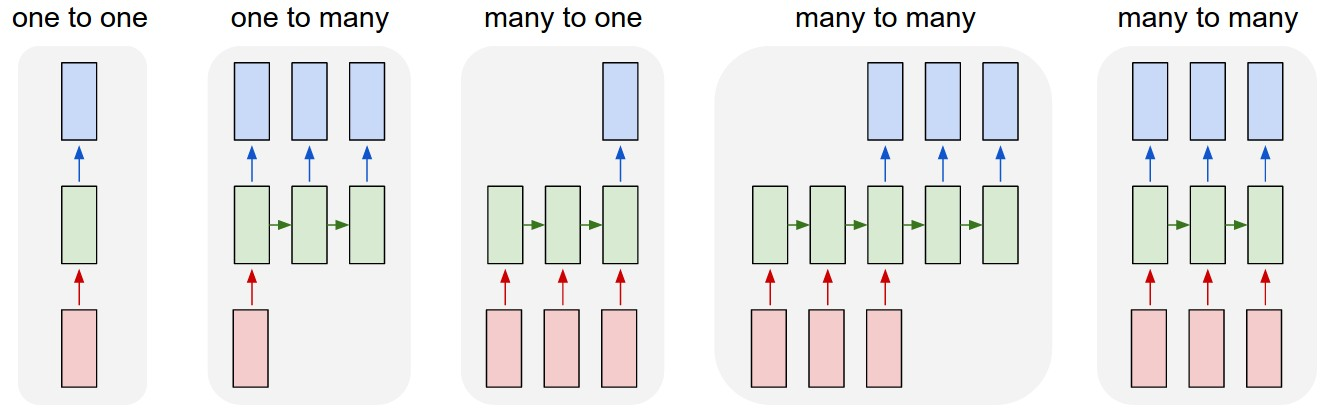
\includegraphics[width=0.5\textwidth]{latex/imgs/rnn_types.png}
    \caption{A visual representation of the output types described. The one-to-one is how fully connected networks work, for comparison. Image Source:\cite{rnn}}
\end{figure}

The basic structure of an RNN is quite simple, consisting of a single linear layer and activation function, which is usually the $tanh$ function. The network is interesting in that each "cell" passes along a hidden state as input to the next cell. This means that each cell takes both the current input element and the previous cell's output and concatenates them and uses this as input to the linear layer.

\begin{figure}[ht]
    \centering
        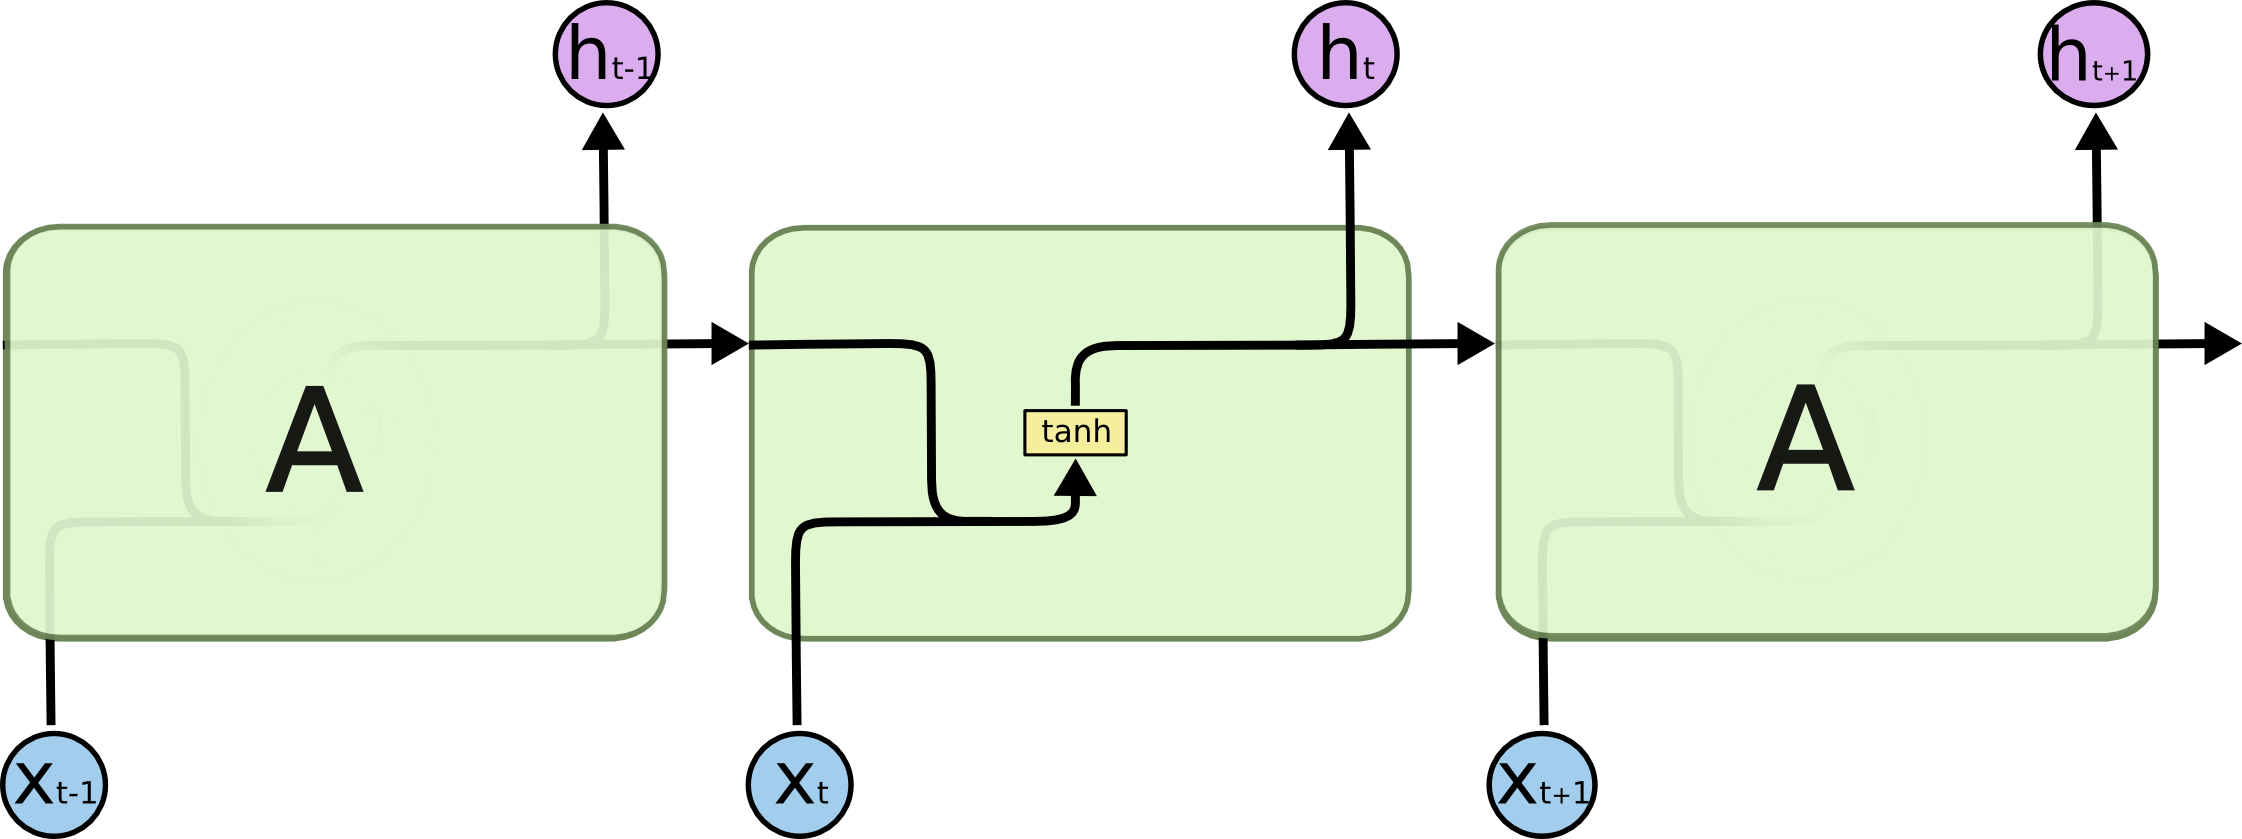
\includegraphics[width=0.5\textwidth]{latex/imgs/rnn.png}
    \caption{A visual representation of the inner structure of an RNN. Image Source:\cite{rnn}}
\end{figure}

\subsubsection{The exploding/vanishing gradient problem}
One major issue with using basic RNNs is the fact that they suffer quite heavily from the exploding/vanishing gradient problem. This problem arises from the fact that very large gradients and gradients very close to zero tend to approach infinity and zero respectively, as they are multiplied together during backpropagation.

To show this, let's consider the following example. We have the prediction vector $h_t$ at each timestep $t$. The gradient when using the backprop through time algorithm looks as follows:
\begin{align}
    \frac{\partial E}{\partial W} = \sum_{t=0}^{T} \frac{\partial E_t}{\partial W}
\end{align}
With network weights $W$ for the concatenated input vectors, and errors $E$ through a sequence of length $T$. We will define the input vectors as follows. $c_t$ for the recurrent vector that the network passes forward, and $x_t$ for the input vector, both at timestep $t$.
This gradient updates the model weights according to the following formula, with a learning rate $\alpha$:
\begin{align}
    W \leftarrow W - \alpha \frac{\partial E}{\partial W}
\end{align}
If we use basic gradient descent, then the gradient of the error at an arbitrary step $s$ is given as follows:
\begin{align}
    \frac{\partial E_s}{\partial W} &= \frac{\partial E_s}{\partial h_s}\frac{\partial h_s}{\partial c_s} \cdots \frac{\partial c_2}{\partial c_1} \frac{\partial c_1}{\partial W} \\
    &= \frac{\partial E_s}{\partial h_s}\frac{\partial h_s}{\partial c_s} \left(\prod_{t=2}^s\frac{\partial c_t}{\partial c_{t-1}} \frac{\partial c_1} {\partial W} \right)
\end{align}
Now we want to show that as $s \rightarrow \infty$ the derivative $\rightarrow 0$. Since the network weights $W$ are the concatenated $c$ and $x$ vectors, we can rewrite $c_t$:
\begin{align}
    c_t = tanh(W_c \cdot c_{t-1} + W_x \cdot x_t)
\end{align}
We find the derivative of this:
\begin{align}
    \frac{\partial c_t}{\partial c_{t-1}} = tanh'(W_c \cdot c_{t-1} + W_x \cdot x_t) \cdot W_c
\end{align}
Plugging these expressions in, we get the following expression:
\begin{align}
    \frac{\partial E_s}{\partial W} &= \frac{\partial E_s}{\partial h_s}\frac{\partial h_s}{\partial c_s} \left(\prod_{t=2}^s tanh'(W_c \cdot c_{t-1} + W_x \cdot x_t) \cdot W_c \right) \frac{\partial c_1}{\partial W}
\end{align}
Since the derivative of the tangent is always strictly $<1$, the expression will tend towards zero as $s \rightarrow \infty$. However, if the weights $W_c$ are significantly large, they may cause the expression to instead explode towards $\infty$ as $s \rightarrow \infty$.\\
\begin{figure}[ht]
    \centering
        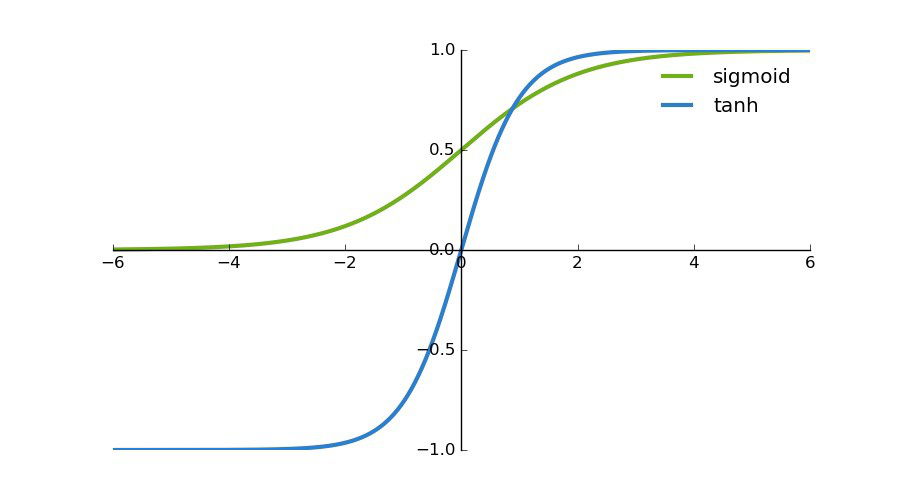
\includegraphics[width=0.75\textwidth]{latex/imgs/tanh_deriv.png}
    \caption{Showing the derivative of the tanh function. Image Source:\cite{grad}}
\end{figure}
If we take a look back at the formula used to update the weights, we can easily see the problem:
\begin{align}
    W &\leftarrow W - \alpha \frac{\partial E}{\partial W}
\end{align}
Since $\frac{\partial E}{\partial W} = \sum_{t=0}^{T} \frac{\partial E_t}{\partial W} \rightarrow 0$ as $T \rightarrow \infty$, we can see that the updates will eventually be incredibly small, to the point where they are basically nonexsistent.

\subsubsection{LSTMs as a solution}
First we will go over how the LSTM architecture works, then we will go over how this solves the vanishing/exploding gradient problem.\\

\noindent
An LSTM actually has an extra input and output vector compared to the base RNN architecture. Much like the base RNN, at time step $t$ it takes an input vector $x_t$ and concatenates it with a hidden vector from a previous output, which we wil refer to as $h_{t-1}$. We will refer to the concatenated vector as $[x_t,h_{t-1}]$. The difference is that it also takes in a cell state, which we will refer to as $c_{t-1}$ since it is also from a previous output. The idea behind this cell state is for it to act as a "highway" for information which can only be changed with linear operations. This means that the cell state is very helpful for remembering information that was learned a long time ago.\\
\begin{figure}[ht]
    \centering
        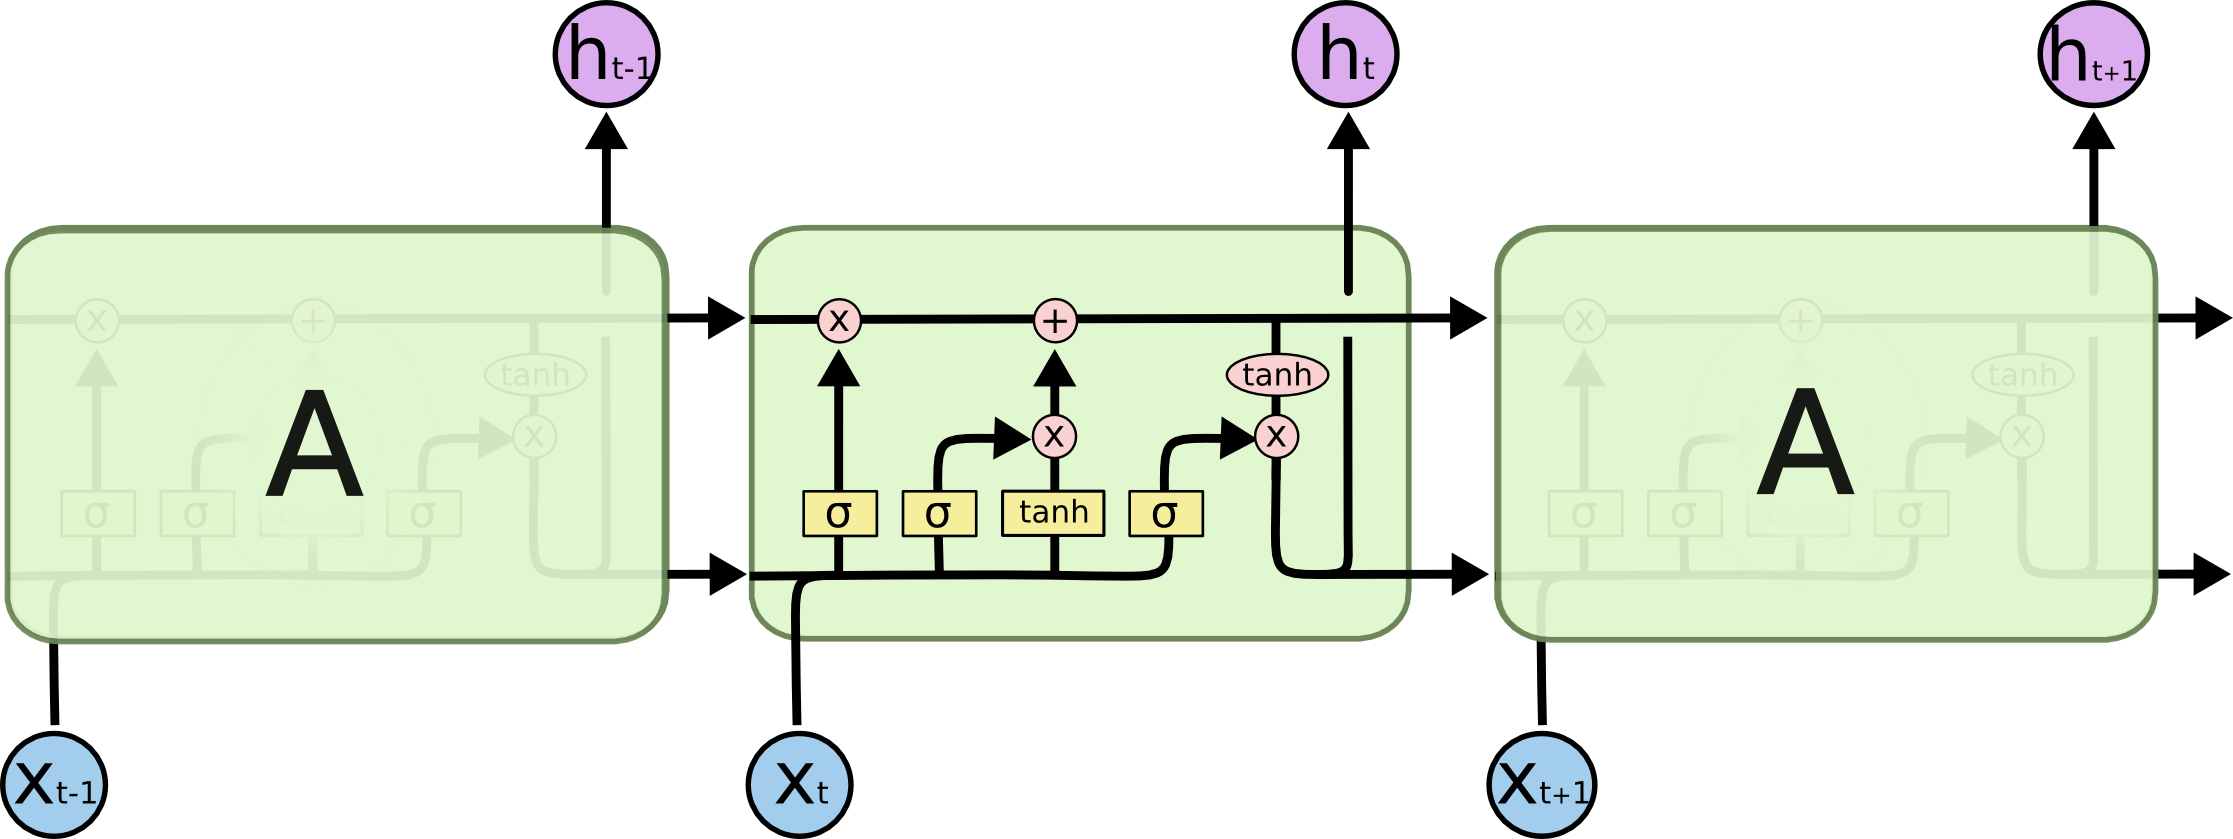
\includegraphics[width=0.75\textwidth]{latex/imgs/lstm.png}
    \caption{Visualisation of the LSTM architecture. Image Source:\cite{lstm}}
    \centering
        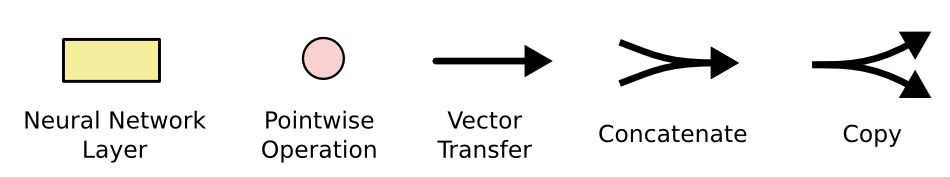
\includegraphics[width=0.5\textwidth]{latex/imgs/lstm_notation.png}
    \caption{Notation for the image above. Image Source:\cite{lstm}}
\end{figure}
Another major difference is the fact that there are four separate linear layers in an LSTM. These layers all take the $[x_t,h_{t-1}]$ vector as input. Going from left to right, we first have the "forget" layer. This layer is activated with a sigmoid function, and controls which parts of the cell state to forget, given new information when training. It is also referred to as a forget "gate" because it controls the information that comes through. It does this by performing pointwise multiplication between the cell state and the output of this layer. The forget gate $f_t$ at time step $t$ with weights $W_f$ is defined mathematically as follows:
\begin{align}
    f_t = \sigma (W_f \cdot [x_t,h_{t-1}])
\end{align}

\noindent
The next two layers also interact with the cell state, but are combined via pointwise multiplication to act as a single gate. The first layer has a sigmoid activation function, while the second has a $tanh$ activation function. The output of this pointwise multiplication will then be combined with the cell state using pointwise addition. This gate acts as an input gate, in the sense that it controls which parts of the cell state get updated as per the new information. With weights $W_c$ for the $tanh$ layer and $W_i$ for the sigmoid layer, the input gate $i_t$ at time step $t$ is defined as follows:
\begin{align}
    i_t &= tanh(W_c \cdot [x_t,h_{t-1}]) \otimes \sigma (W_i \cdot [x_t,h_{t-1}])
\end{align}

\noindent
The final layer also has a sigmoid activation, but is used quite differently. A copy of the cell state will be passed through a tanh activation, and multiplied pointwise with the output of this layer. The output of this is then the new $h_t$ that will be passed forward. This gate acts as an output gate, because it is what controls which parts of the information in the cell state will be passed along as input for the next time step.
With weights $W_o$, the output gate $o_t$ is defined as follows at time step $t$:
\begin{align}
    o_t &= \sigma(W_o \cdot [x_t,h_{t-1}])
\end{align}
The result of all these operations mean that there are two output vectors which are defined as follows:
\begin{align}
    c_t &= c_{t-1} \otimes f_t \oplus i_t \\
    h_t &= \sigma (o_t \otimes tanh (c_t))
\end{align}